\chapter{Project Development}\label{ch:project-development}

This chapter provides an in-depth look into the development of Chronocademy, outlining the key aspects that contributed to its creation.
The following sections will cover essential areas of the project, including product development, user experience, developer experience, the technologies used, and the code architecture.

Each of these areas played a critical role in shaping Chronocademy into a functional and user-friendly platform.
From defining the product's core features and refining its usability to selecting the right tools and structuring the codebase, this chapter highlights the processes and decisions that guided the project from concept to development.

By exploring these topics, the reader will gain a comprehensive understanding of how the team approached the challenges of building Chronocademy and the methods they used to ensure a robust, scalable, and well-designed platform.

\section{Product Development}\label{sec:productdevelopment}
The development of Chronocademy began by defining, refining, and prioritizing its core aspects and features.
This section outlines the step-by-step process undertaken to shape the product, ensuring it was both viable and aligned with the needs of its users.

\subsection{Defining the Idea through the Business Model Canvas}\label{subsec:business-model-canvas}
The first step in the product development journey was to define the core idea behind Chronocademy.
To structure and validate this concept, the team utilized the Business Model Canvas framework.

\begin{quote}
    ``The Business Model Canvas is a strategic management and entrepreneurial tool.
    It allows you to describe, design, challenge, invent, and pivot your business model.
    This method from the bestselling management book Business Model Generation is applied in leading organizations and start-ups worldwide.''
\end{quote}\cite{business-canvas-model}

This tool helped identify the key components of the platform, including the value proposition, target customer segments, revenue streams, cost structure, among others.
By analyzing these elements, the team was able to understand how Chronocademy would create, deliver, and capture value in a competitive landscape.
The structured approach of the Business Model Canvas ensured that the idea was not only innovative but also practical and sustainable.

% Typo in "Adds?" -> "Ads?".
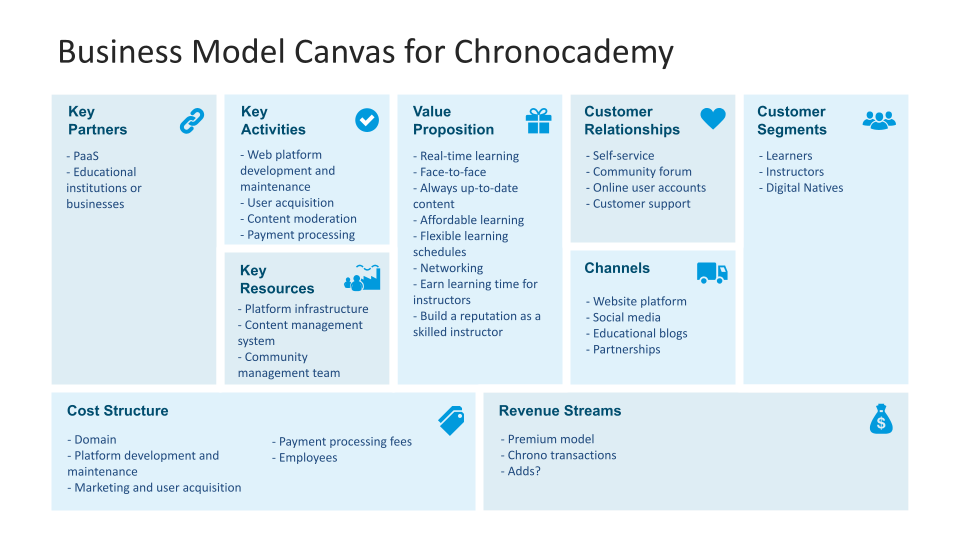
\includegraphics[width=14cm]{business-canvas-model}

\underline{Key resources:}
\begin{itemize}
\item Online platform infrastructure: Website development and maintenance for user accounts, course listings, scheduling, and video conferencing.
\item Content management system (CMS): A system to allow instructors to upload course descriptions and materials.
\item Community management team: Answer to user requests, ensure a positive learning environment and moderate.
\end{itemize}

\underline{Key activities:}
\begin{itemize}
\item Web platform development and maintenance: Develop and continuously update and improve the website for optimal user experience.
\item User acquisition: Marketing strategies to attract users.
\item Content moderation: Moderate courses to ensure quality.
\item Payment processing: Implement a secure system for handling transactions.
\end{itemize}

\underline{Key partnerships:}
\begin{itemize}
\item Video conferencing platform: Integrate a reliable video conferencing service for online lessons.
\item Educational institutions or businesses.
\item Payment processing companies: Integrate a secure payment processor.
\end{itemize}

\underline{Value propositions:}
\begin{itemize}
\item Real-time learning face-to-face: Access to a wide range of skills and knowledge from instructors in real-time face-to-face.
\item Always up-to-date content.
\item Affordable learning: Main payment goes through a time-based exchange system.
\item Flexible learning schedules: Using calendars and through online video conferencing.
\item Networking: Opportunity to connect with a community of learners and instructors.
\item Earn learning time for instructors: Then can be used to acquire new skills and knowledge themselves.
\item Build a reputation as a skilled instructor: Thanks to students feedbacks and ratings.
\end{itemize}

\underline{Customer relationships:}
\begin{itemize}
\item Self-service: Learners and instructors can work autonomous.
\item Community forum: Create a forum for learners and instructors to interact, ask questions, and share experiences.
\item Online user accounts: Users will create accounts to manage their learning time, browse courses, schedule lessons, and provide feedback.
\item Customer support: Offer email or chat support for users encountering technical difficulties, needing assistance or providing feedback.
\end{itemize}

\underline{Customer segment:}
\begin{itemize}
\item Learners: Persons trying to acquire new knowledge through real-time instruction.
\item Instructors: Persons with expertise willing to share their knowledge and earn learning time.
\item Digital natives.
\end{itemize}

\underline{Channels:}
\begin{itemize}
\item Website: Primary channel for user registration, course browsing, lesson scheduling, and video conferencing.
Centralised platform.
\item Social media: Used for marketing, promotion, and building a community around Chronocademy.
\item Educational blogs or partnerships: Collaborate with educational blogs or platforms to promote Chronocademy and reach potential learners.
\end{itemize}

\underline{Cost structure:}
\begin{itemize}
\item Domain: Pay and maintain the internet domain over time.
\item Platform development and maintenance: Costs associated with website development, hosting, and ongoing maintenance.
\item Marketing and user acquisition: Costs for online advertising and social media marketing.
\item Content moderation: Costs associated with managing the course submission process and ensuring lessons quality.
\item Payment processing fees: Fees charged by payment processors for handling transactions.
\item Community management team: Costs associated with management of the online community.
\end{itemize}

\underline{Revenue streams:}
\begin{itemize}
\item Premium model: It offers free Chrono, access to exclusive lessons scripts and a better advertisement for teachers.
\item Chrono transactions: Charge for transactions fees either for buying or selling Chronos.
% Same typo here.
\item Adds: Include adds (not very intrusive).
\end{itemize}

After completing the Business Model Canvas, the team had a clear understanding of the platform's value proposition, target audience, revenue streams, and cost structure.
This work laid the groundwork for the subsequent stages of product development.

\subsection{Establishing the Brand: Colors, Logo, and Slogans}\label{subsec:colors-logo-slogans}
With the foundation of the business model in place, the next focus was on establishing a unique and memorable brand identity for Chronocademy.
The team selected a color palette that reflected the platform’s values of knowledge, reliability and accessibility.
The logo was designed to be simple yet distinctive, incorporating elements that represent time spent on learning and growth.
As well as the name, Chronocademy, which combines the words ``chronos'' (latin for time) and ``academy'' to emphasize the platform's focus on real-time learning.
Slogans were thought to be a good match with the platform, such as ``Learn.
Teach.
Grow.'' These branding efforts were crucial for creating a meaningful identity with the target audience and set Chronocademy apart in the market.

//TODO: this needs refinement, it does not make much sense
\subsubsection{Color Palette}\label{subsubsec:color-palette}
The color palette for Chronocademy was chosen following the colors theory, which is

\begin{quote}
``a set of practices for picking colours together for harmonious designs and contextual combinations''
\end{quote}\cite{colorTheory}.

The first step was to decide which tone of colors would be used, and the team decided to use a mix of pastel colors, which are know for their calming and trustworthy interpretation and some warm colors to give a sense of energy and modern product.

Once this was defined, the team started to work on the style tiles, defined as:

\begin{quote}
``a design deliverable consisting of fonts, colors and interface elements that communicate the essence of a visual brand for the web
[\ldots]
They help form a common visual language between the designers and the stakeholders and provide a catalyst for discussions around the preferences and goals of the client.
[\ldots]
Style tiles establish a direct connection with actual interface elements without defining layout.''
\end{quote}\cite{styleTiles}

The first step to build the style tile board was to define the concept: \textit{``knowledgeable, reliable, and accessible''}.
Then, we searched for images and illustrations that would represent those words and extract the colors out of them.
By doing this a couple of times, we ended up with two different style tiles that were combined to create the final one, by using the fonts of tile number 1 and colors of tile number 2.\newline

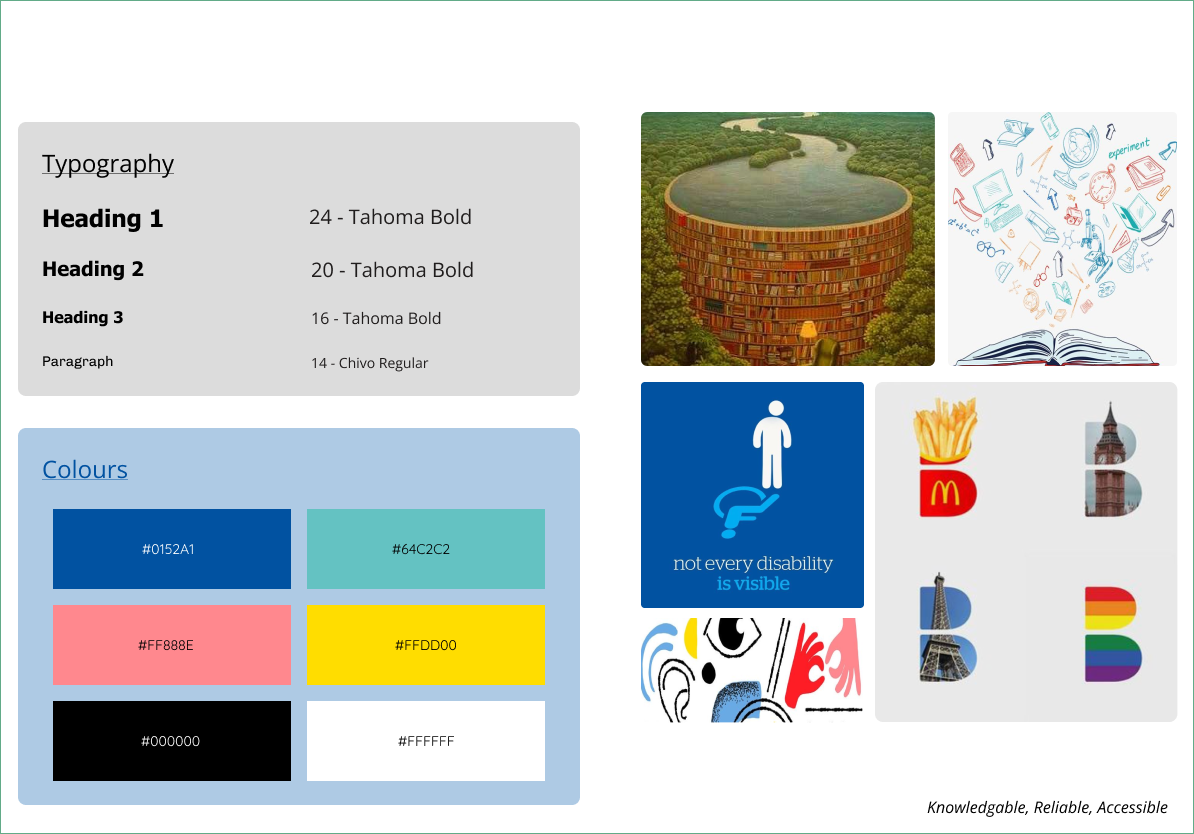
\includegraphics[width=14cm]{style-tile-1}\newline
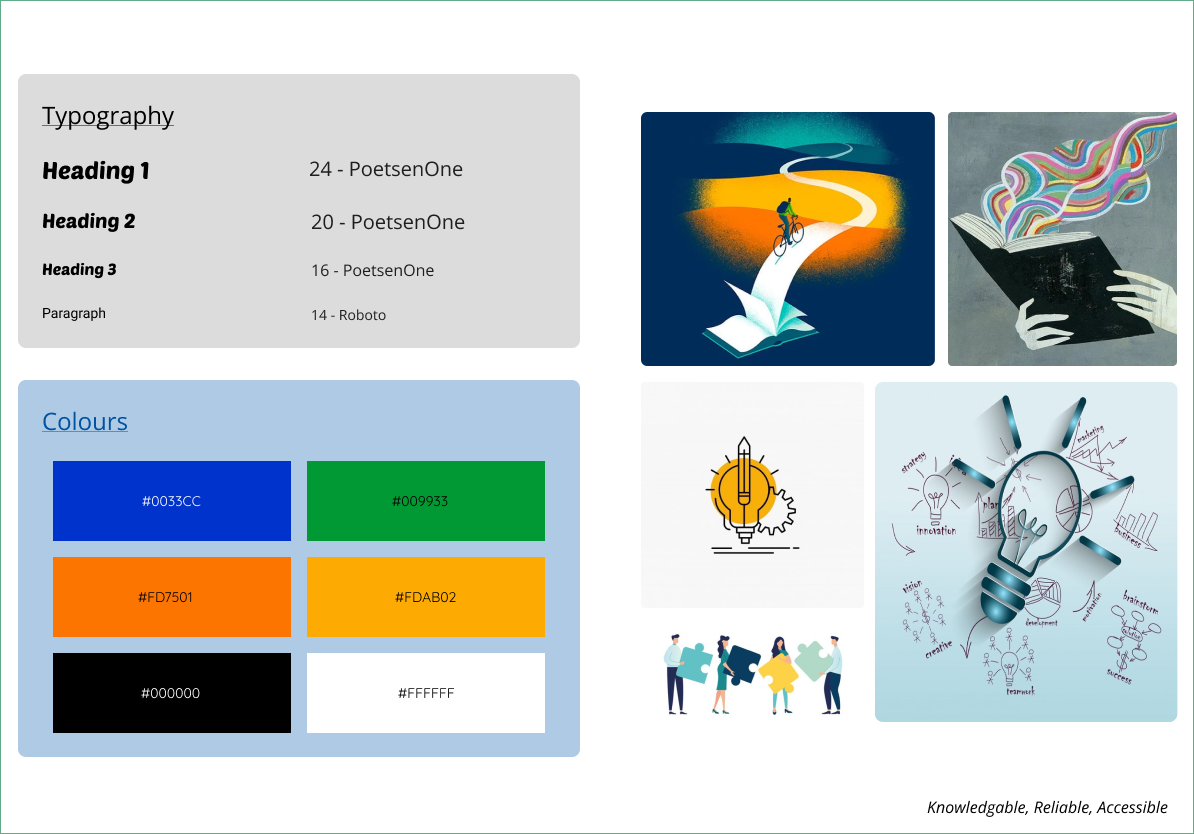
\includegraphics[width=14cm]{style-tile-2}\newline

This tool was helpful to come up with the final color palette and fonts that would be used in the platform.
The final style tile board is shown below.
All three versions were focused on the same concept of \textit{``knowledgeable, reliable, and accessible''}.\newline

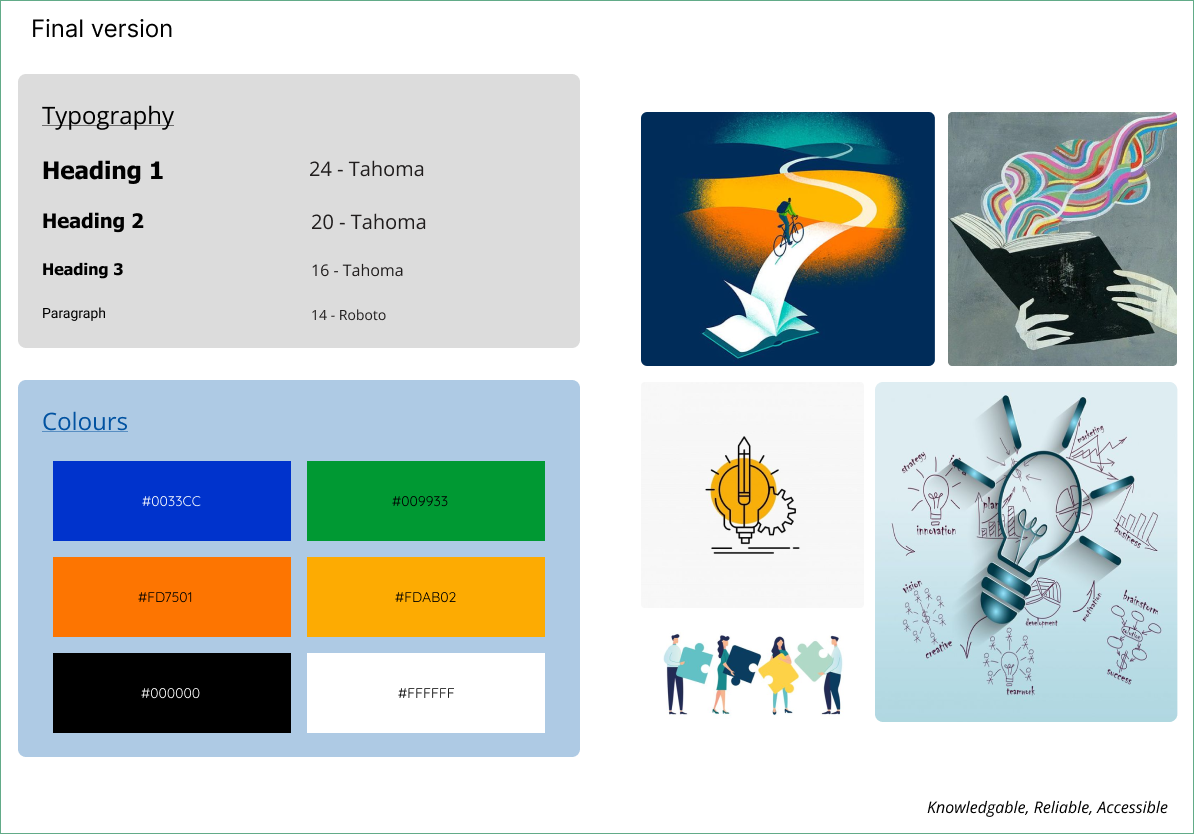
\includegraphics[width=14cm]{style-tile-final}\newline

\subsection{Understanding the Problem: User Interviews and Feature Mapping}\label{subsec:user-interviews-feature-mapping}
To ensure that Chronocademy addressed a real pain / need, the team conducted interviews with potential users.
This exploratory phase involved gathering insights from individuals who were interested in learning new skills or sharing their skills.
The interviews showed common pain points, such as the difficulty of finding reliable teachers, the high cost of learning platforms, and the challenges of managing multiple tools for teaching and learning.
Using the feedback from these interviews, the team mapped user needs into actionable features for the platform.
For instance, the need for affordability led to the time-based currency model, while the desire for better teaching experiences led to the integration of scheduling and video conferencing tools.
This process ensured that every feature of Chronocademy was directly tied to solving a specific user problem.

\subsection{Competitor Analysis}\label{subsec:competitor-analysis}
//TODO: this needs to be filled

\subsection{Prioritizing Features with the Lean Startup Approach}\label{subsec:prioritizing-features-with-the-lean-startup-approach}
Once the features were identified, the team prioritized them using the Minimum Viable Product (MVP) methodology from the Lean Startup approach.
This method emphasized building a version of Chronocademy that included only the essential features needed to deliver value to users and validate the concept.
Features such as the time-based credit system, user profiles, and scheduling integration were classified as high priority and included in the initial release.
% Not sure where these gamification elements came from all of a sudden :D. I feel like they should be mentioned earlier and in depth.
Lower-priority features, such as advanced customization options or gamification elements, were placed on a roadmap for future iterations.
This approach allowed the team to focus on delivering a functional and impactful product in a shorter time frame while leaving room for growth and improvement based on user feedback.
